% Cross-machine transfer figure: grouped bar chart
% FD002 / FD003 / FD004 RMSE for V2 (causal) vs V16a (bidi) vs V16b (bidi+VICReg)
% Data source: experiments/v16/phase4_cross_machine_results.json
%
% Story: causal V2 wins on cross-machine transfer; bidirectional variants overfit
% to FD001 and transfer worse. Visual evidence for the causal inductive bias finding.

\documentclass[border=8pt]{standalone}
\usepackage{tikz}
\usepackage{amsmath,amssymb}
\usetikzlibrary{
  arrows.meta, positioning, shapes.geometric,
  fit, calc, decorations.pathreplacing, backgrounds,
  patterns.meta
}
% Forgis brand colors — academic palette for white-background figures
% Source: color_schema.json
%
% Usage: % Forgis brand colors — academic palette for white-background figures
% Source: color_schema.json
%
% Usage: % Forgis brand colors — academic palette for white-background figures
% Source: color_schema.json
%
% Usage: \input{colors.tex} in each standalone figure .tex file.
% All figures MUST use only these colors. No inline hex.

% Brand primaries
\definecolor{ctiger}{HTML}{FF5A00}       % Primary accent (Forgis orange)
\definecolor{cfire}{HTML}{FF4D00}        % Critical
\definecolor{cflicker}{HTML}{DC4B07}     % Secondary accent
\definecolor{csteel}{HTML}{878F92}       % Muted neutral
\definecolor{cgunmetal}{HTML}{122128}    % Dark text

% Academic derived palette
\definecolor{cprimary}{HTML}{FF5A00}     % = tiger
\definecolor{cprimarylight}{HTML}{FF8C42}
\definecolor{cprimarybg}{HTML}{FFF0E6}
\definecolor{csecondary}{HTML}{2B6CB0}   % Complementary blue
\definecolor{csecondarylight}{HTML}{4A90D9}
\definecolor{csecondarybg}{HTML}{E8F0FA}
\definecolor{caccent}{HTML}{2D8A6E}      % Teal
\definecolor{caccentlight}{HTML}{5BB89A}
\definecolor{caccentbg}{HTML}{E6F5F0}
\definecolor{chighlight}{HTML}{DC4B07}   % = flicker
\definecolor{chighlightbg}{HTML}{FDEDE6}
\definecolor{ctextdark}{HTML}{122128}    % = gunmetal
\definecolor{ctextmid}{HTML}{878F92}     % = steel
\definecolor{ctextlight}{HTML}{B0B7BA}
\definecolor{cborder}{HTML}{D1D5D8}
\definecolor{cbgwarm}{HTML}{FFF8F2}
\definecolor{cbgcool}{HTML}{F4F7FA}
 in each standalone figure .tex file.
% All figures MUST use only these colors. No inline hex.

% Brand primaries
\definecolor{ctiger}{HTML}{FF5A00}       % Primary accent (Forgis orange)
\definecolor{cfire}{HTML}{FF4D00}        % Critical
\definecolor{cflicker}{HTML}{DC4B07}     % Secondary accent
\definecolor{csteel}{HTML}{878F92}       % Muted neutral
\definecolor{cgunmetal}{HTML}{122128}    % Dark text

% Academic derived palette
\definecolor{cprimary}{HTML}{FF5A00}     % = tiger
\definecolor{cprimarylight}{HTML}{FF8C42}
\definecolor{cprimarybg}{HTML}{FFF0E6}
\definecolor{csecondary}{HTML}{2B6CB0}   % Complementary blue
\definecolor{csecondarylight}{HTML}{4A90D9}
\definecolor{csecondarybg}{HTML}{E8F0FA}
\definecolor{caccent}{HTML}{2D8A6E}      % Teal
\definecolor{caccentlight}{HTML}{5BB89A}
\definecolor{caccentbg}{HTML}{E6F5F0}
\definecolor{chighlight}{HTML}{DC4B07}   % = flicker
\definecolor{chighlightbg}{HTML}{FDEDE6}
\definecolor{ctextdark}{HTML}{122128}    % = gunmetal
\definecolor{ctextmid}{HTML}{878F92}     % = steel
\definecolor{ctextlight}{HTML}{B0B7BA}
\definecolor{cborder}{HTML}{D1D5D8}
\definecolor{cbgwarm}{HTML}{FFF8F2}
\definecolor{cbgcool}{HTML}{F4F7FA}
 in each standalone figure .tex file.
% All figures MUST use only these colors. No inline hex.

% Brand primaries
\definecolor{ctiger}{HTML}{FF5A00}       % Primary accent (Forgis orange)
\definecolor{cfire}{HTML}{FF4D00}        % Critical
\definecolor{cflicker}{HTML}{DC4B07}     % Secondary accent
\definecolor{csteel}{HTML}{878F92}       % Muted neutral
\definecolor{cgunmetal}{HTML}{122128}    % Dark text

% Academic derived palette
\definecolor{cprimary}{HTML}{FF5A00}     % = tiger
\definecolor{cprimarylight}{HTML}{FF8C42}
\definecolor{cprimarybg}{HTML}{FFF0E6}
\definecolor{csecondary}{HTML}{2B6CB0}   % Complementary blue
\definecolor{csecondarylight}{HTML}{4A90D9}
\definecolor{csecondarybg}{HTML}{E8F0FA}
\definecolor{caccent}{HTML}{2D8A6E}      % Teal
\definecolor{caccentlight}{HTML}{5BB89A}
\definecolor{caccentbg}{HTML}{E6F5F0}
\definecolor{chighlight}{HTML}{DC4B07}   % = flicker
\definecolor{chighlightbg}{HTML}{FDEDE6}
\definecolor{ctextdark}{HTML}{122128}    % = gunmetal
\definecolor{ctextmid}{HTML}{878F92}     % = steel
\definecolor{ctextlight}{HTML}{B0B7BA}
\definecolor{cborder}{HTML}{D1D5D8}
\definecolor{cbgwarm}{HTML}{FFF8F2}
\definecolor{cbgcool}{HTML}{F4F7FA}


\begin{document}
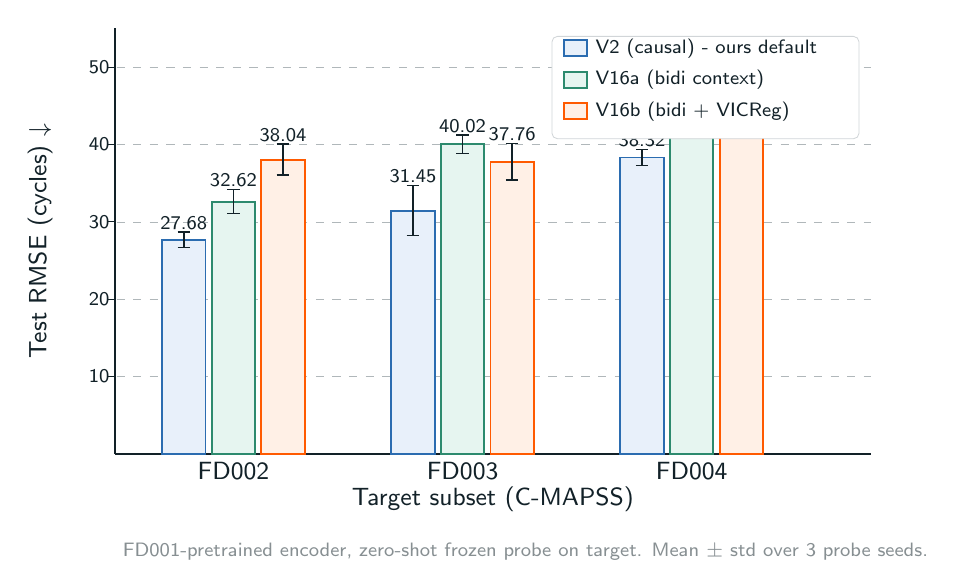
\begin{tikzpicture}[
  font=\sffamily\small,
  every node/.style={inner sep=0pt, outer sep=0pt},
]

% ========================================================
% Axes: x = FD002, FD003, FD004 groups; y = RMSE
% Data (mean RMSE on test set, 3 probe seeds):
%   FD002: V2=27.68, V16a=32.62, V16b=38.04
%   FD003: V2=31.45, V16a=40.02, V16b=37.76
%   FD004: V2=38.32, V16a=43.60, V16b=49.66
% Max value ~= 50 -> y-axis: 0 to 55 with ticks at 0, 10, 20, 30, 40, 50.
% ========================================================

% Layout constants
\def\plotw{9.6}   % plot area width (cm)
\def\ploth{5.4}   % plot area height (cm)
\def\ymax{55}     % data max for y-axis

% y-axis scaling: 1 RMSE unit = \ploth / \ymax cm
\pgfmathsetmacro{\yscale}{\ploth / \ymax}

% Bar and group widths
\def\bw{0.55}     % single bar width (cm)
\def\bgap{0.08}   % gap between bars within a group (cm)
\def\ggap{1.1}    % gap between groups (cm)

% One group = 3 bars + 2 internal gaps
\pgfmathsetmacro{\groupw}{3*\bw + 2*\bgap}

% Axes origin
\coordinate (O) at (0,0);

% y-axis line
\draw[ctextdark, line width=0.6pt] (O) -- ++(0,\ploth);
% x-axis line
\draw[ctextdark, line width=0.6pt] (O) -- ++(\plotw,0);

% y-axis ticks and labels (every 10 RMSE)
\foreach \y in {10,20,30,40,50} {
  \pgfmathsetmacro{\ypos}{\y * \yscale}
  \draw[ctextdark, line width=0.4pt] (0, \ypos) -- ++(-0.10,0);
  \node[left=2pt, ctextdark] at (0, \ypos) {\scriptsize \y};
  % faint gridline
  \draw[ctextlight, line width=0.2pt, dashed] (0.02, \ypos) -- (\plotw, \ypos);
}

% y-axis title (rotated)
\node[rotate=90, ctextdark, anchor=center] at (-0.95, \ploth/2)
  {Test RMSE (cycles) $\downarrow$};

% ========================================================
% Groups: FD002, FD003, FD004
% Left edge of first group:
\def\gleft{0.6}

% Group data: {name, v2, v16a, v16b, v2std, v16astd, v16bstd}
\def\dataFDtwo{{27.68, 32.62, 38.04}}
\def\stdFDtwo{{1.00, 1.54, 2.01}}
\def\dataFDthree{{31.45, 40.02, 37.76}}
\def\stdFDthree{{3.26, 1.22, 2.36}}
\def\dataFDfour{{38.32, 43.60, 49.66}}
\def\stdFDfour{{1.00, 1.46, 1.70}}

% Colors per method:
%   V2     : csecondary (blue)     causal
%   V16a   : caccent (teal)        bidi
%   V16b   : cprimary (orange)     bidi + VICReg

% Helper: draw group at x-offset \xg with data array \dat, std \estd, label \glab
% (we inline for clarity)

% ─── FD002 group ───
\pgfmathsetmacro{\gx}{\gleft}
\foreach \i/\col/\val/\stdv in {0/csecondary/27.68/1.00, 1/caccent/32.62/1.54, 2/cprimary/38.04/2.01} {
  \pgfmathsetmacro{\bx}{\gx + \i * (\bw + \bgap)}
  \pgfmathsetmacro{\by}{\val * \yscale}
  \pgfmathsetmacro{\eby}{(\val + \stdv) * \yscale}
  \pgfmathsetmacro{\ebl}{(\val - \stdv) * \yscale}
  % filled bar (secondary_bg / accent_bg / primary_bg), darker border
  \pgfmathsetmacro{\bxmid}{\bx + \bw/2}
  \ifnum\i=0
    \fill[csecondarybg] (\bx, 0) rectangle (\bx+\bw, \by);
  \fi
  \ifnum\i=1
    \fill[caccentbg] (\bx, 0) rectangle (\bx+\bw, \by);
  \fi
  \ifnum\i=2
    \fill[cprimarybg] (\bx, 0) rectangle (\bx+\bw, \by);
  \fi
  \draw[\col, line width=0.7pt] (\bx, 0) rectangle (\bx+\bw, \by);
  % error bar
  \draw[ctextdark, line width=0.5pt] (\bxmid, \ebl) -- (\bxmid, \eby);
  \draw[ctextdark, line width=0.5pt] (\bxmid-0.08, \eby) -- (\bxmid+0.08, \eby);
  \draw[ctextdark, line width=0.5pt] (\bxmid-0.08, \ebl) -- (\bxmid+0.08, \ebl);
  % value label above error bar
  \node[above=1pt, ctextdark, font=\sffamily\scriptsize] at (\bxmid, \eby) {\val};
}
\pgfmathsetmacro{\gmid}{\gx + \groupw/2}
\node[below=3pt, ctextdark] at (\gmid, 0) {FD002};

% ─── FD003 group ───
\pgfmathsetmacro{\gx}{\gleft + \groupw + \ggap}
\foreach \i/\col/\val/\stdv in {0/csecondary/31.45/3.26, 1/caccent/40.02/1.22, 2/cprimary/37.76/2.36} {
  \pgfmathsetmacro{\bx}{\gx + \i * (\bw + \bgap)}
  \pgfmathsetmacro{\by}{\val * \yscale}
  \pgfmathsetmacro{\eby}{(\val + \stdv) * \yscale}
  \pgfmathsetmacro{\ebl}{(\val - \stdv) * \yscale}
  \pgfmathsetmacro{\bxmid}{\bx + \bw/2}
  \ifnum\i=0
    \fill[csecondarybg] (\bx, 0) rectangle (\bx+\bw, \by);
  \fi
  \ifnum\i=1
    \fill[caccentbg] (\bx, 0) rectangle (\bx+\bw, \by);
  \fi
  \ifnum\i=2
    \fill[cprimarybg] (\bx, 0) rectangle (\bx+\bw, \by);
  \fi
  \draw[\col, line width=0.7pt] (\bx, 0) rectangle (\bx+\bw, \by);
  \draw[ctextdark, line width=0.5pt] (\bxmid, \ebl) -- (\bxmid, \eby);
  \draw[ctextdark, line width=0.5pt] (\bxmid-0.08, \eby) -- (\bxmid+0.08, \eby);
  \draw[ctextdark, line width=0.5pt] (\bxmid-0.08, \ebl) -- (\bxmid+0.08, \ebl);
  \node[above=1pt, ctextdark, font=\sffamily\scriptsize] at (\bxmid, \eby) {\val};
}
\pgfmathsetmacro{\gmid}{\gx + \groupw/2}
\node[below=3pt, ctextdark] at (\gmid, 0) {FD003};

% ─── FD004 group ───
\pgfmathsetmacro{\gx}{\gleft + 2*(\groupw + \ggap)}
\foreach \i/\col/\val/\stdv in {0/csecondary/38.32/1.00, 1/caccent/43.60/1.46, 2/cprimary/49.66/1.70} {
  \pgfmathsetmacro{\bx}{\gx + \i * (\bw + \bgap)}
  \pgfmathsetmacro{\by}{\val * \yscale}
  \pgfmathsetmacro{\eby}{(\val + \stdv) * \yscale}
  \pgfmathsetmacro{\ebl}{(\val - \stdv) * \yscale}
  \pgfmathsetmacro{\bxmid}{\bx + \bw/2}
  \ifnum\i=0
    \fill[csecondarybg] (\bx, 0) rectangle (\bx+\bw, \by);
  \fi
  \ifnum\i=1
    \fill[caccentbg] (\bx, 0) rectangle (\bx+\bw, \by);
  \fi
  \ifnum\i=2
    \fill[cprimarybg] (\bx, 0) rectangle (\bx+\bw, \by);
  \fi
  \draw[\col, line width=0.7pt] (\bx, 0) rectangle (\bx+\bw, \by);
  \draw[ctextdark, line width=0.5pt] (\bxmid, \ebl) -- (\bxmid, \eby);
  \draw[ctextdark, line width=0.5pt] (\bxmid-0.08, \eby) -- (\bxmid+0.08, \eby);
  \draw[ctextdark, line width=0.5pt] (\bxmid-0.08, \ebl) -- (\bxmid+0.08, \ebl);
  \node[above=1pt, ctextdark, font=\sffamily\scriptsize] at (\bxmid, \eby) {\val};
}
\pgfmathsetmacro{\gmid}{\gx + \groupw/2}
\node[below=3pt, ctextdark] at (\gmid, 0) {FD004};

% x-axis title below group labels
\node[below=12pt, ctextdark] at (\plotw/2, 0) {Target subset (C-MAPSS)};

% ========================================================
% Legend (top-right area, inside plot)
% ========================================================
\def\legx{5.7}
\def\legy{5.05}
% Legend box (subtle)
\draw[cborder, line width=0.3pt, fill=white, rounded corners=2pt]
  (\legx-0.15, \legy-1.05) rectangle (\legx + 3.75, \legy+0.25);

% V2 (causal)
\fill[csecondarybg] (\legx, \legy) rectangle ++(0.3, 0.2);
\draw[csecondary, line width=0.7pt] (\legx, \legy) rectangle ++(0.3, 0.2);
\node[right=3pt, ctextdark, font=\sffamily\scriptsize, anchor=west]
  at (\legx+0.3, \legy+0.1) {V2 (causal) - ours default};

% V16a (bidi)
\fill[caccentbg] (\legx, \legy-0.4) rectangle ++(0.3, 0.2);
\draw[caccent, line width=0.7pt] (\legx, \legy-0.4) rectangle ++(0.3, 0.2);
\node[right=3pt, ctextdark, font=\sffamily\scriptsize, anchor=west]
  at (\legx+0.3, \legy-0.3) {V16a (bidi context)};

% V16b (bidi + VICReg)
\fill[cprimarybg] (\legx, \legy-0.8) rectangle ++(0.3, 0.2);
\draw[cprimary, line width=0.7pt] (\legx, \legy-0.8) rectangle ++(0.3, 0.2);
\node[right=3pt, ctextdark, font=\sffamily\scriptsize, anchor=west]
  at (\legx+0.3, \legy-0.7) {V16b (bidi + VICReg)};

% ========================================================
% Source note (bottom-left, small)
% ========================================================
\node[font=\sffamily\scriptsize, ctextmid, anchor=south west]
  at (0.1, -1.35) {FD001-pretrained encoder, zero-shot frozen probe on target. Mean $\pm$ std over 3 probe seeds.};

\end{tikzpicture}
\end{document}
